\documentclass{article}
\usepackage[utf8]{inputenc}
\usepackage[dutch]{babel}
\usepackage[square,sort,comma,numbers]{natbib}
\usepackage[hyphens]{url}
\usepackage{tikz}
\usetikzlibrary{trees}
\usepackage{float}
\usepackage{hyperref}
\setlength
{\parindent}
{0pt}
\setlength
{\parskip}
{1.5ex plus 0.5ex minus 0.2ex}
\usepackage[margin=3.5cm]{geometry}


\title{Artificiële Intelligentie: Opdracht 3 (STRIPS Planning)}
\author{Mathias Van Herreweghe - r0456156}
\date{12 december 2014}

\usepackage{natbib}
\usepackage{graphicx}

\begin{document}

\maketitle
\newpage

\section{Opgave}
Op een lesvrije dag besef je dat het belangrijk is dat je fiets in orde wordt gemaakt. Het blijft namelijk steeds minder lang licht. Je besluit dus dat je best naar de Velo (fiets-herstelpunt) gaat waar je gratis kan gebruik maken van hun gereedschap. De onderdelen heb je vooraf bij hun besteld en betaald. Deze liggen klaar bij Velo zelf om gebruikt te worden. Voor je vertrekt besluit je dat het een goed idee is om deze herstelling te plannen, dit is uiteraard mogelijk met behulp van het STRIPS planning algoritme.

De toezichter van de herstelplaats geeft je nog de tip mee dat je best de band direct na binnenband hersteld. Dit omdat dus eigenlijk twee handelingen (operatoren) in één bezigheid, je kan echter nog steeds materiaal nemen tussen het maken van de binnenband en de band.

\subsection{Initiële situatie en doel-situatie}

\begin{figure}[H]
\centering
\begin{tabular}{|c|l|}
    \multicolumn{2}{c}{Initiële situatie}\\
    \hline
    if & \\
    \hline
    add & In(Kot)\\
    \hline
    del & \\
    \hline
\end{tabular}
\hspace{0.25 cm}
\begin{tabular}{|c|l|}
    \multicolumn{2}{c}{Doel-situatie}\\
    \hline
    if & In(Kot)\\
       & Fiets(Hersteld)\\
    \hline
    add & \\
    \hline
    del & \\
    \hline
\end{tabular}
\caption{Initiële situatie en doel-situatie}
\label{initialfinal_s}
\end{figure}

Figuur \ref{initialfinal_s} laat zien wat de initiële situatie en de doel-situatie inhoudt. Initieel ben je in je kot en is je fiets kapot. De doel-situatie is dat je terug op je kot bent en je fiets hersteld is.

\subsection{Mogelijke operatoren}

\begin{figure}[H]
\centering
\begin{tabular}{|c|c|}
    \multicolumn{2}{c}{Naar herstelplaats (NH)}\\
    \hline
    if & In(Kot)\\
    \hline
    add & In(Herstelplaats)\\
        & Vrij(Handen)\\
    \hline
    del & In(Kot)\\
    \hline
\end{tabular}
\hspace{0.25cm}
\begin{tabular}{|c|c|}
    \multicolumn{2}{c}{Neem fietslicht (NF)}\\
    \hline
    if & In(Herstelplaats)\\
    \hline
    add & Heeft(Fietslicht)\\
    \hline
    del & \\
    \hline
\end{tabular}
\\\vspace{0.25cm}
\begin{tabular}{|c|c|}
    \multicolumn{2}{c}{Neem band (NB)}\\
    \hline
    if & In(Herstelplaats)\\
    \hline
    add & Heeft(Band)\\
    \hline
    del & \\
    \hline
\end{tabular}
\hspace{0.25cm}
\begin{tabular}{|c|c|}
    \multicolumn{2}{c}{Neem binnenband (NBB)}\\
    \hline
    if & In(Herstelplaats)\\
    \hline
    add & Heeft(Binnenband)\\
    \hline
    del & \\
    \hline
\end{tabular}
\\\vspace{0.25cm}
\begin{tabular}{|c|c|}
    \multicolumn{2}{c}{Herstel fietslicht (HF)}\\
    \hline
    if & In(Herstelplaats)\\
       & Vrij(Handen)\\
       & Heeft(Fietslicht)\\
    \hline
    add & Hersteld(Fietslicht)\\
    \hline
    del & Heeft(Fietslicht)\\
    \hline
\end{tabular}
\hspace{0.25cm}
\begin{tabular}{|c|c|}
    \multicolumn{2}{c}{Herstel binnenband (HBB)}\\
    \hline
    if & In(Herstelplaats)\\
       & Vrij(Handen)\\
       & Heeft(Binnenband)\\
    \hline
    add & Hersteld(Binnenband)\\
    \hline
    del & Vrij(Handen)\\
        & Heeft(Binnenband)\\
    \hline
\end{tabular}
\\\vspace{0.25cm}
\begin{tabular}{|c|c|}
    \multicolumn{2}{c}{Herstel band (HB)}\\
    \hline
    if & In(Herstelplaats)\\
       & Heeft(Band)\\
       & Hersteld(Binnenband)\\
    \hline
    add & Hersteld(Band)\\
        & Vrij(Handen)\\
    \hline
    del & Heeft(Band)\\
    \hline
\end{tabular}
\hspace{0.25cm}
\begin{tabular}{|c|c|}
    \multicolumn{2}{c}{Naar kot (NK)}\\
    \hline
    if & In(Herstelplaats)\\
    \hline
    add & In(Kot)\\
    \hline
    del & In(Herstelplaats)\\
        & Vrij(Handen)\\
    \hline
\end{tabular}
\\\vspace{0.25cm}
\begin{tabular}{|c|c|}
    \multicolumn{2}{c}{Controleer fiets (CF)}\\
    \hline
    if & In(Herstelplaats)\\
       & Hersteld(Fietslicht)\\
       & Hersteld(Binnenband)\\
       & Hersteld(Band)\\
    \hline
    add & Hersteld(Fiets)\\
    \hline
    del & Hersteld(Fietslicht)\\
        & Hersteld(Binnenband)\\
        & Hersteld(Band)\\
    \hline
\end{tabular}
\caption{Mogelijke acties}
\label{acties}
\end{figure}

\newpage
\section{Model oplossing}

\subsection{Establishes- en threatens-graaf}

Op figuur \ref{E_T_Graaf} zie je een graaf met de initiële situatie, de doelsituatie en alle acties. Alle establish links zijn aangeduid in een groene kleur, threatens links in het rood.

\begin{figure}[H]
\centering
\caption{Establish- en threatens-links graaf}
\label{E_T_Graaf}
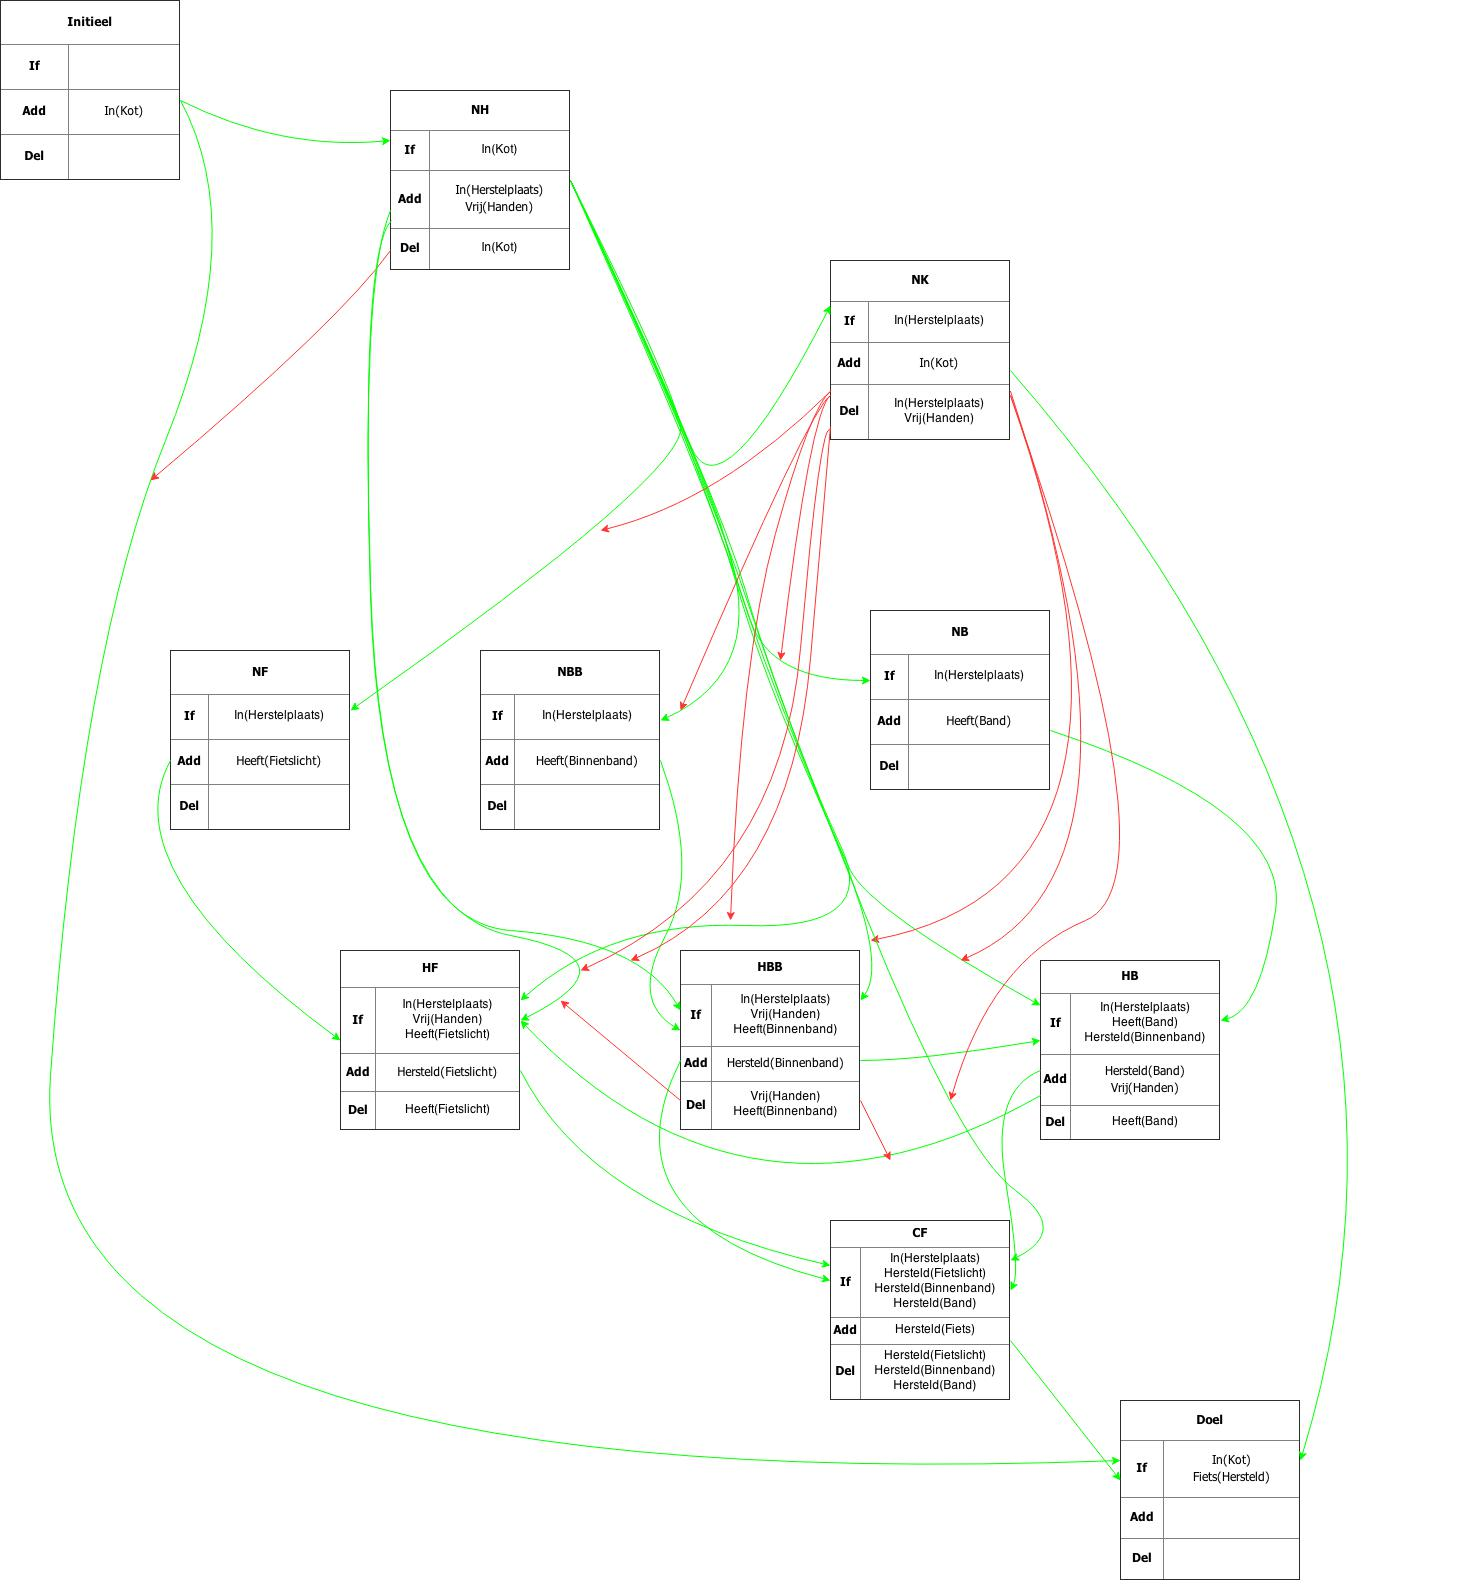
\includegraphics[scale=0.2791]{Est_Thr_Graaf.jpg}
\end{figure}

\newpage
\subsection{Before-graaf}

In figuur \ref{Before-graaf} is de graaf weergeven met al de before-relaties. Deze laat zien welke handelingen voor andere handelingen moeten uitgevoerd worden.

\begin{figure}[H]
\centering
\caption{Before-graaf}
\label{Before-graaf}
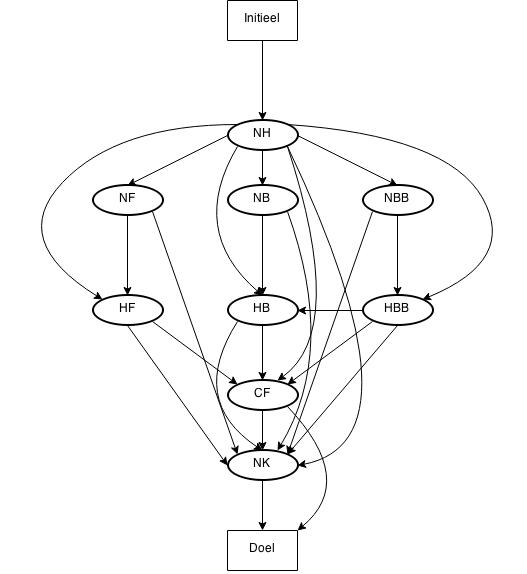
\includegraphics[scale=0.5]{Before_graaf.jpg}
\end{figure}

\newpage
\subsection{Mogelijke plannen}

Aan de hand van figuur \ref{Before-graaf} kan eveneens een opsomming worden gemaakt van alle mogelijke plannen. Zo zijn er uiteraard verschillende mogelijkheden in de volgorden van wanneer je de de verschillende banden en het fietslicht neemt, en deze vervolgens hersteld. Deze mogelijkheden worden hieronder weergegeven\footnote{Deze mogelijkheden zijn gegenereerd door een zelfgemaakt algoritme in Java omdat dit manueel teveel werk zou zijn.}.

\[
\begin{array}{c}
Initieel \rightarrow NF \rightarrow HF \rightarrow NB \rightarrow NBB \rightarrow HBB \rightarrow HB \rightarrow CF \rightarrow NK \rightarrow Doel\\
Initieel \rightarrow NF \rightarrow HF \rightarrow NBB \rightarrow NB \rightarrow HBB \rightarrow HB \rightarrow CF \rightarrow NK \rightarrow Doel\\
Initieel \rightarrow NF \rightarrow HF \rightarrow NBB \rightarrow HBB \rightarrow NB \rightarrow HB \rightarrow CF \rightarrow NK \rightarrow Doel\\
Initieel \rightarrow NF \rightarrow NB \rightarrow HF \rightarrow NBB \rightarrow HBB \rightarrow HB \rightarrow CF \rightarrow NK \rightarrow Doel\\
Initieel \rightarrow NF \rightarrow NB \rightarrow NBB \rightarrow HF \rightarrow HBB \rightarrow HB \rightarrow CF \rightarrow NK \rightarrow Doel\\
Initieel \rightarrow NF \rightarrow NB \rightarrow NBB \rightarrow HBB \rightarrow HB \rightarrow HF \rightarrow CF \rightarrow NK \rightarrow Doel\\
Initieel \rightarrow NF \rightarrow NBB \rightarrow HF \rightarrow NB \rightarrow HBB \rightarrow HB \rightarrow CF \rightarrow NK \rightarrow Doel\\
Initieel \rightarrow NF \rightarrow NBB \rightarrow HF \rightarrow HBB \rightarrow NB \rightarrow HB \rightarrow CF \rightarrow NK \rightarrow Doel\\
Initieel \rightarrow NF \rightarrow NBB \rightarrow NB \rightarrow HF \rightarrow HBB \rightarrow HB \rightarrow CF \rightarrow NK \rightarrow Doel\\
Initieel \rightarrow NF \rightarrow NBB \rightarrow NB \rightarrow HBB \rightarrow HB \rightarrow HF \rightarrow CF \rightarrow NK \rightarrow Doel\\
Initieel \rightarrow NF \rightarrow NBB \rightarrow HBB \rightarrow NB \rightarrow HB \rightarrow HF \rightarrow CF \rightarrow NK \rightarrow Doel\\
Initieel \rightarrow NB \rightarrow NF \rightarrow HF \rightarrow NBB \rightarrow HBB \rightarrow HB \rightarrow CF \rightarrow NK \rightarrow Doel\\
Initieel \rightarrow NB \rightarrow NF \rightarrow NBB \rightarrow HF \rightarrow HBB \rightarrow HB \rightarrow CF \rightarrow NK \rightarrow Doel\\
Initieel \rightarrow NB \rightarrow NF \rightarrow NBB \rightarrow HBB \rightarrow HB \rightarrow HF \rightarrow CF \rightarrow NK \rightarrow Doel\\
Initieel \rightarrow NB \rightarrow NBB \rightarrow NF \rightarrow HF \rightarrow HBB \rightarrow HB \rightarrow CF \rightarrow NK \rightarrow Doel\\
Initieel \rightarrow NB \rightarrow NBB \rightarrow NF \rightarrow HBB \rightarrow HB \rightarrow HF \rightarrow CF \rightarrow NK \rightarrow Doel\\
Initieel \rightarrow NB \rightarrow NBB \rightarrow HBB \rightarrow NF \rightarrow HB \rightarrow HF \rightarrow CF \rightarrow NK \rightarrow Doel\\
Initieel \rightarrow NB \rightarrow NBB \rightarrow HBB \rightarrow HB \rightarrow NF \rightarrow HF \rightarrow CF \rightarrow NK \rightarrow Doel\\
Initieel \rightarrow NBB \rightarrow NF \rightarrow HF \rightarrow NB \rightarrow HBB \rightarrow HB \rightarrow CF \rightarrow NK \rightarrow Doel\\
Initieel \rightarrow NBB \rightarrow NF \rightarrow HF \rightarrow HBB \rightarrow NB \rightarrow HB \rightarrow CF \rightarrow NK \rightarrow Doel\\
Initieel \rightarrow NBB \rightarrow NF \rightarrow NB \rightarrow HF \rightarrow HBB \rightarrow HB \rightarrow CF \rightarrow NK \rightarrow Doel\\
Initieel \rightarrow NBB \rightarrow NF \rightarrow NB \rightarrow HBB \rightarrow HB \rightarrow HF \rightarrow CF \rightarrow NK \rightarrow Doel\\
Initieel \rightarrow NBB \rightarrow NF \rightarrow HBB \rightarrow NB \rightarrow HB \rightarrow HF \rightarrow CF \rightarrow NK \rightarrow Doel\\
Initieel \rightarrow NBB \rightarrow NB \rightarrow NF \rightarrow HF \rightarrow HBB \rightarrow HB \rightarrow CF \rightarrow NK \rightarrow Doel\\
Initieel \rightarrow NBB \rightarrow NB \rightarrow NF \rightarrow HBB \rightarrow HB \rightarrow HF \rightarrow CF \rightarrow NK \rightarrow Doel\\
Initieel \rightarrow NBB \rightarrow NB \rightarrow HBB \rightarrow NF \rightarrow HB \rightarrow HF \rightarrow CF \rightarrow NK \rightarrow Doel\\
Initieel \rightarrow NBB \rightarrow NB \rightarrow HBB \rightarrow HB \rightarrow NF \rightarrow HF \rightarrow CF \rightarrow NK \rightarrow Doel\\
Initieel \rightarrow NBB \rightarrow HBB \rightarrow NF \rightarrow NB \rightarrow HB \rightarrow HF \rightarrow CF \rightarrow NK \rightarrow Doel\\
Initieel \rightarrow NBB \rightarrow HBB \rightarrow NB \rightarrow NF \rightarrow HB \rightarrow HF \rightarrow CF \rightarrow NK \rightarrow Doel\\
Initieel \rightarrow NBB \rightarrow HBB \rightarrow NB \rightarrow HB \rightarrow NF \rightarrow HF \rightarrow CF \rightarrow NK \rightarrow Doel\\
\end{array}
\]

\end{document}
